\chapter{Manual de usuario}

\textbf{Pantalla de inicio de HIVmlm}
\begin{figure}[H]
\centering
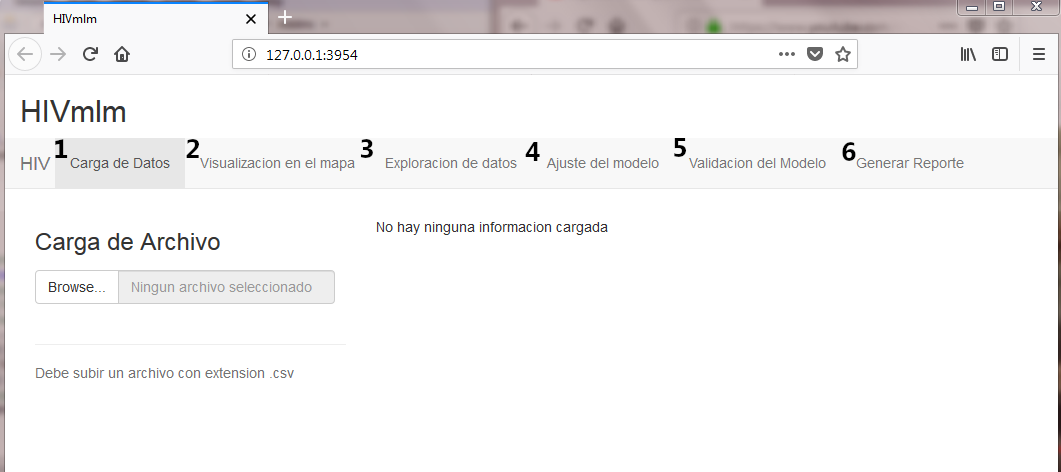
\includegraphics[scale=0.5]{inicio.PNG}
\caption{Pantalla de inicio de HIVmlm}
\end{figure}

\begin{enumerate}
\item \textbf{Carga de datos:} Modulo de carga del archivo
\item \textbf{Visualizaci\'on en el mapa:} Muestra la incidencia del virus en el mapa
\item \textbf{Exploraci\'on de datos:} Muestra el analisis grafico de los datos cargados
\item \textbf{Ajuste del Modelo:} Analisis del modelo lineal mixto
\item \textbf{Validaci\'on del modelo:} Muestra graficamente los datos obtenidos del modelo lineal mixto.
\item \textbf{Generar reporte:} Permite generar reportes con los datos de la aplicaci\'on 
\end{enumerate}

 \noindent
\textbf{M\'odulo de carga de datos}

\begin{figure}[H]
\centering
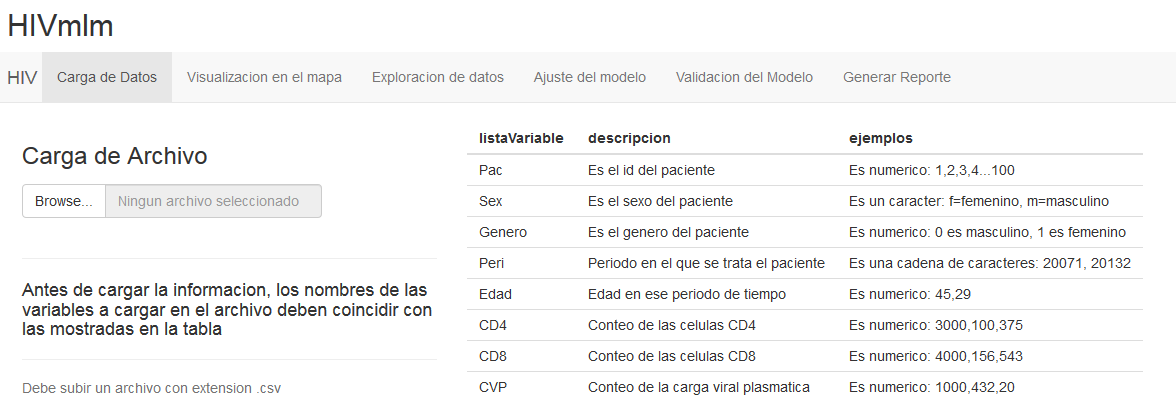
\includegraphics[scale=0.5]{cargaArchivo.PNG}
\caption{Pantalla de la carga del archivo}
\end{figure}

 \noindent
\textbf{Carga de datos}

Para cargar el archivo, se debe hace click en \textbf{Browse} como lo muestra la figura B.3.

\begin{figure}[H]
\centering
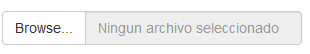
\includegraphics[scale=0.8]{browse.PNG}
\caption{Carga de archivo en la aplicaci\'on}
\end{figure}

Posteriormente se mostrar\'a una ventana para seleccionar el archivo como se muestra en la figura B.4.

\begin{figure}[H]
\centering
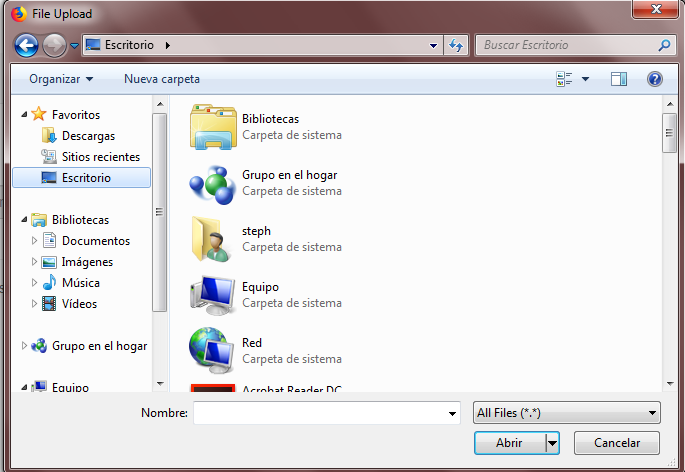
\includegraphics[scale=0.5]{fileup.PNG}
\caption{Selecci\'on del archivo a cargar}
\end{figure}

Se mostrar\'a la informaci\'on en la aplicaci\'on.

\begin{figure}[H]
\centering
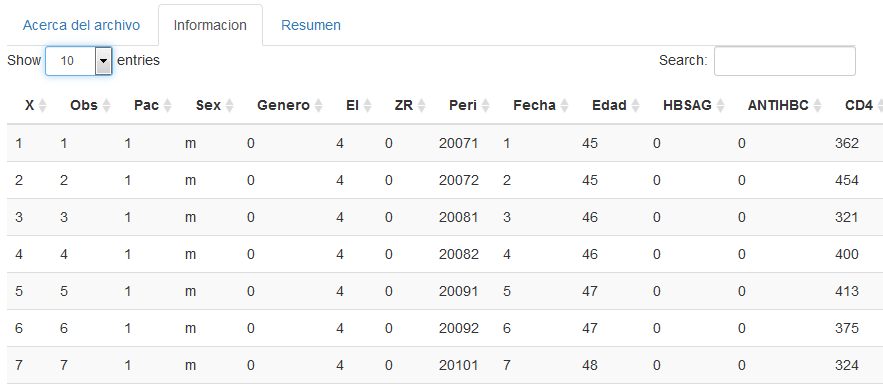
\includegraphics[scale=0.6]{Cargafile2.PNG}
\caption{Informaci\'on del archivo}
\end{figure}

Luego se puede navegar en la aplicaci\'on, con los diferentes modulos, para la exploraci\'on y el analisis de los datos.\\

 \noindent
\textbf{M\'odulo de visualizaci\'on del mapa}

En este m\'odulo, se detalla en el mapa, la incidencia de la ubicaci\'on y el contagio del virus en la localidad.

\begin{figure}[H]
  \centering
  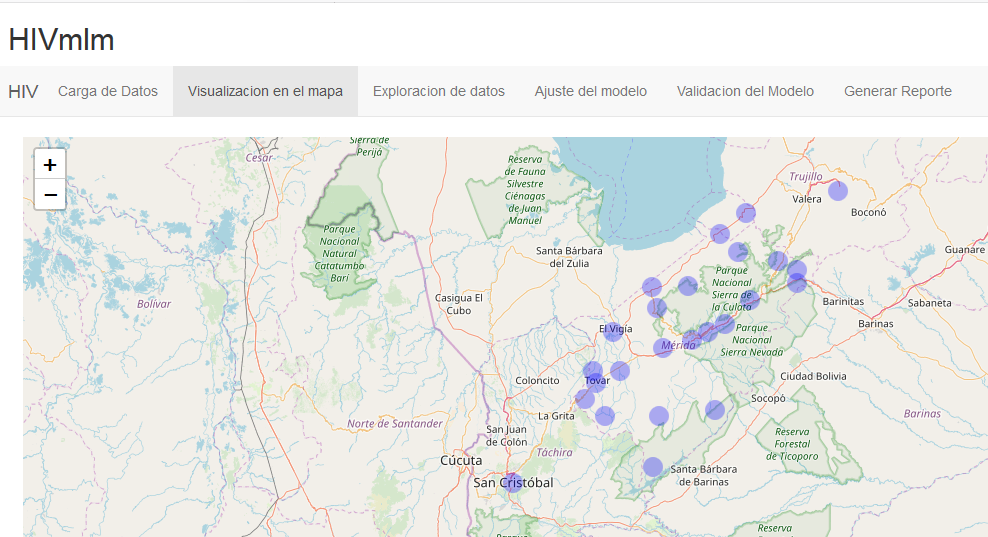
\includegraphics[scale=0.6]{mapa1.PNG}
   \caption{Pantalla de la visualizaci\'on del mapa}
  \end{figure}
  
Al presionar o darle click a los puntos azules ubicados en el mapa, se puede visualizar la informaci\'on realtiva a la media de la carga viral plasmatica y las c\'elulas CD4, n\'umero de pacientes, g\'enero, desviaci\'on estandar y tiempo medio de duraci\'on.

\begin{figure}[H]
\centering
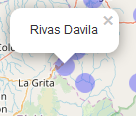
\includegraphics[scale=0.8]{mapa2.PNG}
\caption{Selecci\'on de un punto azul sobre el mapa}
\end{figure}

\textbf{M\'odulo de Exploraci\'on de datos}

En el siguiente m\'odulo, esta dividido en 3 paneles, es decir, el genero, la edad y las cargas. 

\begin{figure}[H]
\centering
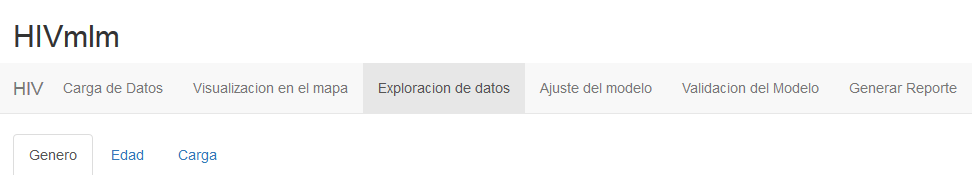
\includegraphics[scale=0.6]{explorar.PNG}
\caption{Visualizaci\'on del m\'odulo de Exploraci\'on de datos}
\end{figure}

En la siguiente figura, se puede visualizar que en la secci\'on \textbf{g\'enero} hay un selector por per\'iodo, en este caso, se puede seleccionar entre 20071 hasta 20132, obteniendo el siguiente gr\'afico.

\begin{figure}[H]
\centering
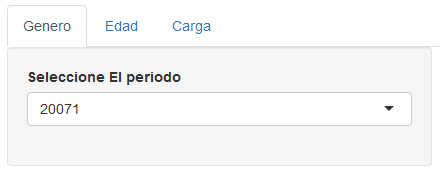
\includegraphics[scale=0.6]{panel.PNG}
\caption{Pantalla de los 3 paneles para visualizar graficamente los datos}
\end{figure}

\begin{figure}[H]
\centering
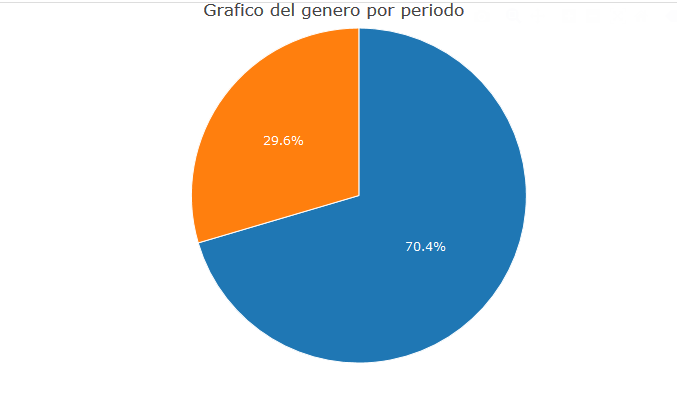
\includegraphics[scale=0.6]{genero.PNG}
\caption{Visualizaci\'on de la gr\'afica de torta por g\'enero}
\end{figure}

En la secci\'on \textbf{Edad} muestra un histograma como lo muestra la siguiente figura B.11

\begin{figure}[H]
\centering
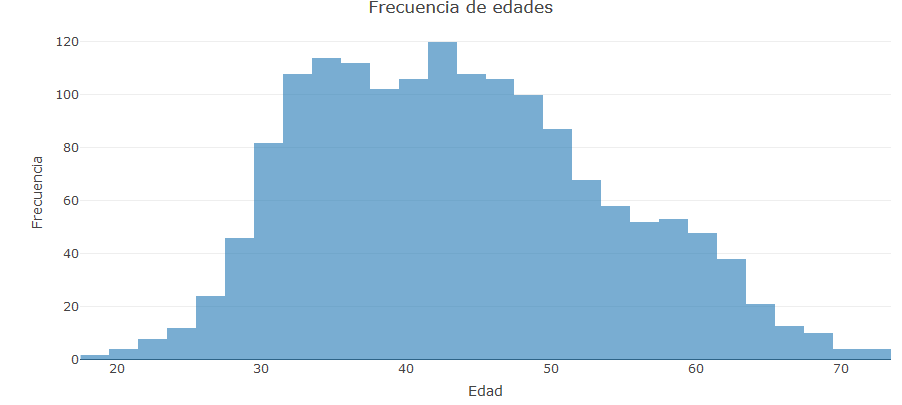
\includegraphics[scale=0.6]{edad.PNG}
\caption{Pantalla con el histograma de edades}
\end{figure}

En la secci\'on \textbf{Cargas} muestra un selector, con las variables Carga Viral plasmatica, celulas $T^{+}CD4$ y $T^{+}CD8$. Permite visualizar un gr\'afico de puntos.

\begin{figure}[H]
\centering
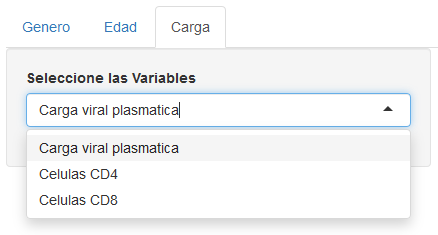
\includegraphics[scale=0.6]{exploraCarg.PNG}
\caption{Pantalla del selector de la secci\'on cargas}
\end{figure}

\begin{figure}[H]
\centering
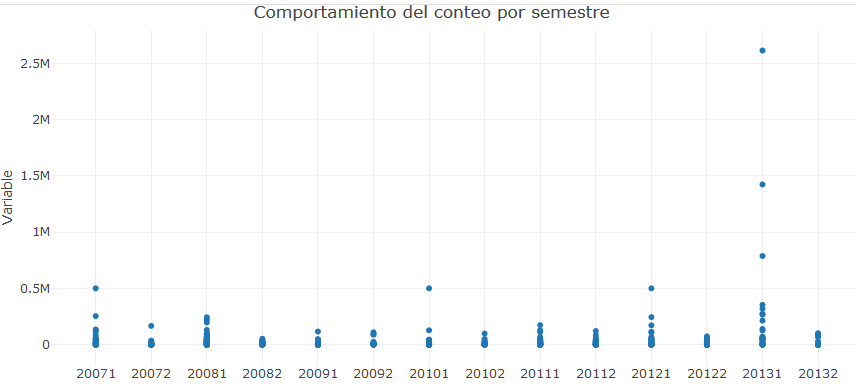
\includegraphics[scale=0.6]{CVP.PNG}
\caption{Visualizaci\'on del gr\'afico de puntos}
\end{figure}

 \noindent
\textbf{M\'odulo Ajuste del modelo}

En este m\'odulo, muestra la implementaci\'on del modelo lineal mixto.

\begin{figure}[H]
\centering
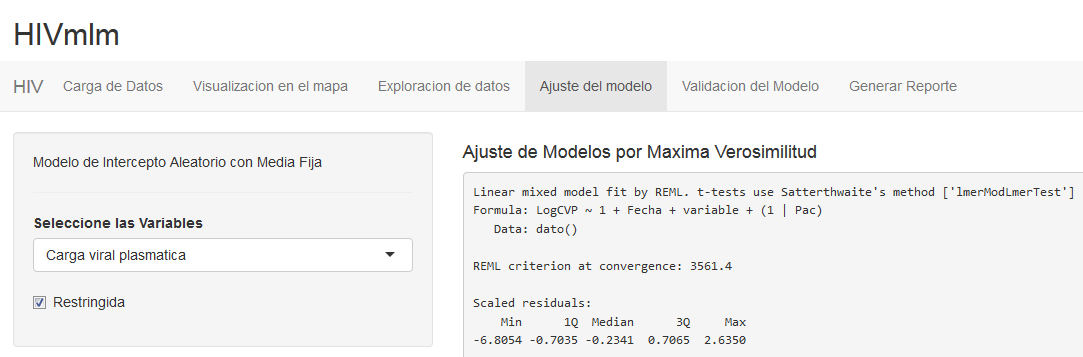
\includegraphics[scale=0.5]{ajusteModel.PNG}
\caption{Pantalla con el m\'odulo ajuste del modelo}
\end{figure}

Contiene un selector que permite seleccionar entre las variables carga viral plasm\'atica, c\'elulas $T^{+}CD4$ y $T^{+}CD8$ y un cuadro de selecci\'on, con la variable Restingida, permitiendo variar el modelo matem\'atico.

\begin{figure}[H]
\centering
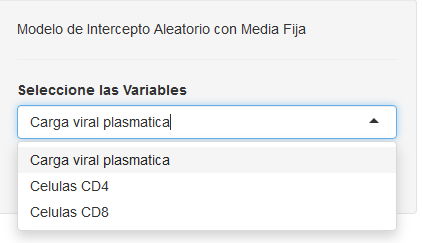
\includegraphics[scale=0.6]{cuadrosele.PNG}
\caption{Pantalla con el selector del m\'odulo de ajuste del modelo}
\end{figure}

Luego de seleccionar las variables, sale la siguiente informaci\'on como lo muestra la figura B.16.

\begin{figure}[H]
\centering
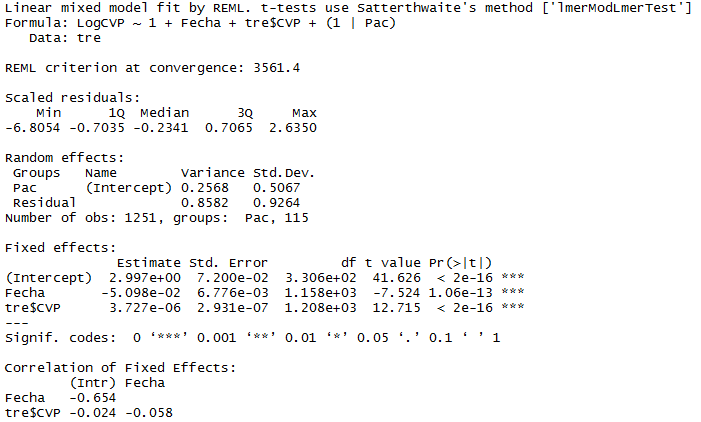
\includegraphics[scale=0.6]{lme.png}
\caption{Pantalla con la informaci\'on del modelo lineal mixto}
\end{figure}

 \noindent
\textbf{M\'odulo de validaci\'on del modelo}

En este m\'odulo, muestra el resultado de los residuos, calculados en el m\'odulo anterior, el ajuste del modelo, lo que permite visualizar el comportamiento de los datos en el modelo lineal mixto. Permite seleccionar entre las variables Carga viral plasmatica, celulas $T^{+}CD4$ y $T^{+}CD8$.

\begin{figure}[H]
\centering
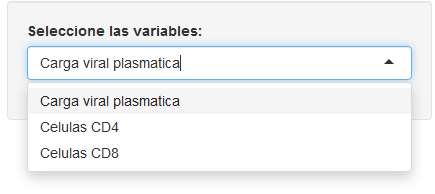
\includegraphics[scale=0.6]{valido2.PNG}
\caption{Pantalla selecci\'on de las variables de la validaci\'on del modelo}
\end{figure}

Genera la siguiente gr\'afica.

\begin{figure}[H]
\centering
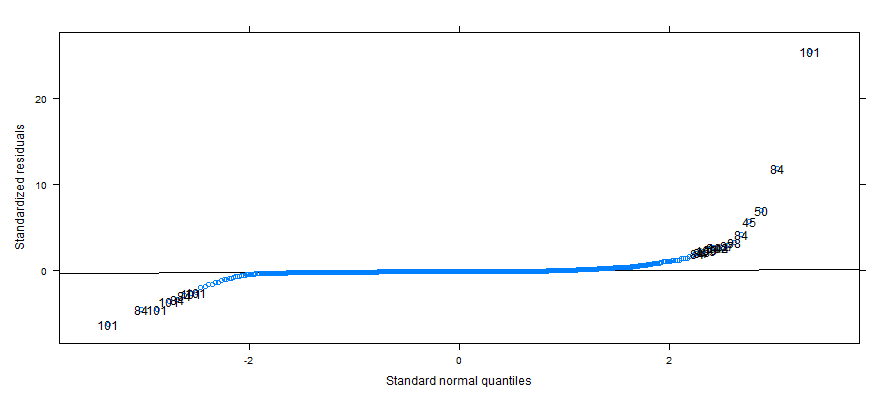
\includegraphics[scale=0.6]{valido.PNG}
\caption{Gr\'afica de la validaci\'on del modelo}
\end{figure}

\textbf{M\'odulo generar reporte}

En este m\'odulo, permite generar el reporte de las graficas y el an\'alisis del modelo lineal mixto. Aparece un boton de descargar reporte, se le da click.

\begin{figure}[H]
\centering
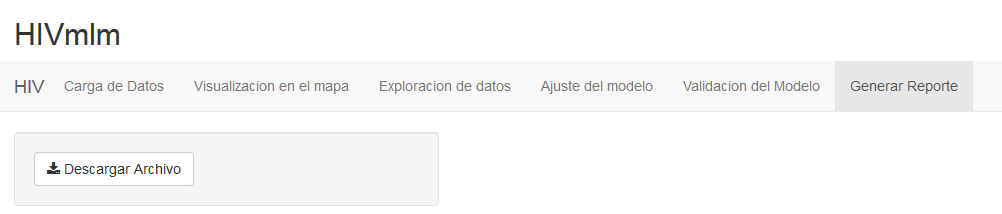
\includegraphics[scale=0.6]{reporte2.PNG}
\caption{Pantalla del bot\'on de descarga del reporte}
\end{figure}

Luego aparece una ventana, donde permite guardar el reporte, se le da click en ok, y lo guarda.

\begin{figure}[H]
\centering
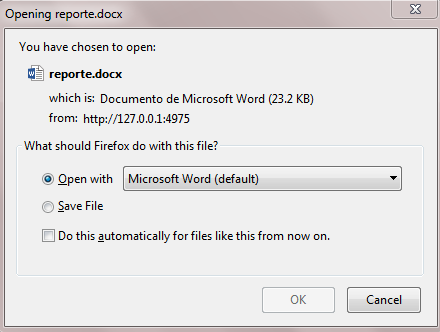
\includegraphics[scale=0.6]{reporte3.PNG}
\caption{Pantalla de guardar el reporte}
\end{figure}









    

